\chapter{Introdução}
\label{cap:introducao}

A internet das coisas segundo \cite{Ashton} refere-se a convergência tecnológica onde as coisas do mundo real, ou seja, objetos usados no nosso dia-a-dia estarão conectados entre si e a rede de mundial de computadores. Nesse novo mundo as ``coisas” conectadas passarão a ser mais inteligentes, coletar informações ao seu redor e realizar tarefas automaticamente sem a interferência humana. \\
\indent Em meio aos vários objetos que aos poucos estão dando forma a internet das coisas estão os beacons. Beacons são pequenos dispositivos que utilizam a tecnologia bluetooth para detectar a presença de outros dispositivos (smartphones, tablets, etc), dentro do seu raio, que também tenham bluetooth ativo e iniciar uma ação nesses mesmos dispositivos através de um aplicativo intermediário previamente instalado. \\
\indent Os beacons podem agir de forma ativa, permitindo que as aplicações com que eles interagem, possam prover aos usuários informações com base no seu contexto de localização. Ou de forma passiva simplesmente registrando que um determinado dispositivo entrou em seu raio de detecção, esses registros podem ser trabalhados por outros sistemas para obter a localização aproximada do usuário em relação ao beacon. \\
\indent A aplicabilidade dos beacons são diversas. Podem ser utilizados para mapeamento de fluxo de usuários em shoppings, feiras e eventos diversos; localização em ambientes fechados (indoor); ou em uma loja de varejo, enviar uma notificação com informação de ofertas de produtos para os smartphones de clientes quando eles passarem por uma determinada área da loja. Também existem outras possibilidades, como: checkins automáticos e até pagamentos através de dispositivos móveis.



\section{Problema}
\label{sec:problema}

Segundo \cite{Teixeira} beacons não são inteligentes, toda a inteligência fica sob responsabilidade do aplicativo instalado no dispositivo que irá interagir com o beacon. Atualmente no mercado existem dois padrões principais para comunicação entre beacons e aplicações, o iBeacon criando e mantido pela Apple, é um padrão proprietário que funciona somente com os dispositivos da própria fabricante e o Eddystone criando e mantido pela Google, é um padrão aberto (open-source) que pode ser utilizado por qualquer dispositivo. Em ambos os padrões o beacon age conforme a afirmação anterior, a total dependência de uma aplicação pode representar um problema em alguns casos, como por exemplo no cenário em que uma loja de varejo deseja utilizar beacons para prover informações para os seus clientes com base nos dados de seus próprios perfis e também histórico das últimas compras realizadas, que estão armazenados em seus servidores de banco de dados, mas não deseja disponibilizar por razões de segurança, um serviço público que exponha os dados dos clientes diretamente para um aplicativo. \\
\indent Neste último cenário seria mais seguro que os dados podessem ser tratados, caso fosse necessário, pelo próprio beacon antes de serem enviados para a aplicação instalada no dispositivo do cliente que está interagindo com ele. Além disso, o acesso do serviço sendo realizado através do beacon representa mais segurança para a rede interna da loja, pois neste cenário o beacon é um dispositivo que pode ser controlado pelo próprio administrador da rede.

\section{Objetivos}
\label{sec:objetivos}

Neste tópico serão abordados os objetivos geral e específicos desta monografia.

\subsection{Objetivo Geral}
\label{sec:objetivo-geral}

Desenvolver um protótipo de sistema de beacon baseado na tecnologia wifi para aumentar a taxa de transferência de dados e a segurança de aplicações baseadas em beacons bluetooth.

\subsection{Objetivos Específicos}
\label{sec:objetivos-especificos}

	\begin{itemize}
		\item Pesquisar e definir as tecnologias, ferramentas e suas configurações para criar o beacon wifi;
		\item Implementar o algoritmo do protocolo de comunicação para o beacon e os dispositivos;
		\item Desenvolver o aplicativo cliente para comunicação;
		\item Desenvolver um serviço para prover as informações para o sistema utilizando o beacon e o aplicativo cliente;
		\item Validar o protótipo quanto ao aumento da taxa de transferência de dados e segurança.
	\end{itemize}

\section{Justificativa}
\label{sec:justificativa}

Seguindo o propósito da internet das coisas, em disponibilizar dispositivos cada vez mais inteligentes que possam executar tarefas automaticamente sem a intervenção humana, este trabalho tem o intuito de desenvolver um beacon capaz não somente de detectar a presença dos dispositivos que entrarem em seu raio de ação, mas também um beacon mais inteligente que os encontrados atualmente no mercado, podendo processar dados internamente e também comunicar diretamente com serviços internos ou externos.

\section{Trabalhos Relacionados}
\label{sec:trabalhos-relacionados}

\cite{ChoiParkLee} descreveram um sistema de gerenciamento de energia de escritório capaz de reduzir o consumo de energia de computadores, monitores e luzes de um escritório com a utilização de beacons baseados em bluetooth e um aplicativo móvel. Enquanto vários beacons foram colocados em lugares estratégicos do escritório de forma a cobrir todos os espaços, um aplicativo móvel determina, com a ajuda dos beacons, se o usuário entrou ou saiu do escritório e modificam o modo de economia de energia dos computadores, monitores e luzes. O sistema proposto pode reduzir o consumo de energia em um escritório sem causar desconforto aos usuários. No caso da utilização de beacons wifi, com um único dispositivo, seria possível cobrir toda uma sala do escritório. \\
\indent \cite{Bohonos} descreveram um sistema de software e hardware chamado URNA (Universal Real-Time Navigational Assistance) que permite a comunicação de informações relevantes de localização para uma pessoa cega através de um celular com bluetooth. O sistema tem como alvo principal ajudar um pedestre cego na travessia de ruas de um cruzamento, informando o nome da rua e o estado atual do semáforo. Com o uso de beacon wifi, visto que a tecnologia bluetooth tem um curto alcance, o sistema poderia ser estendido com a criação de um aplicativo para os motoristas, cuja a funcionalidade seria comunicar com o beacon e informá-los sobre a presença de pedestres cegos a medida que o mesmo se aproximasse de um semáforo. \\
\indent \cite{Chawathe} descreve um método de localização de dispositivos móveis em ambientes fechados usando beacons baseados em bluetooth. Nesse caso o raio de detecção limitado da tecnologia bluetooth é usado como vantagem. Mas para isso é preciso estabelecer de forma correta a posição de cada beacon, de modo que os beacons não sofram com interferência de raio de outro beacon.

\section{Método de Investigação}
\label{sec:metodo-investigacao}

A metodologia de desenvolvimento proposta para este trabalho é composta das seguintes etapas: \\
\indent A pesquisa de referencial teórico sobre beacons será baseada nas principais fontes encontradas no mercado e/ou disponibilizado na internet, como livros, artigos, tutoriais e revistas. Com intuito de fornecer ao trabalho um embasamento teórico necessário para o entendimento dos beacons, os conceitos envolvidos e suas características. \\
\indent A pesquisa de tecnologias e ferramentas necessárias para definição da arquitetura e construção de um beacon baseado na tecnologia wifi utilizando o microcomputador Raspberry Pi, juntamente com seu sistema operacional raspbian baseado na distribuição linux debian. Bem como a forma de detecção dos dispositivos cliente; e também o protocolo de comunicação a ser utilizado entre o beacon e esses dispositivos. \\
\indent Na etapa de desenvolvimento serão implementados: o protótipo do aplicativo cliente que fará uso das principais ferramentas encontradas para o desenvolvimento android, sendo o Android Studio como ambiente integrado de desenvolvimento (IDE) e o Framework Android; e o serviço responsável por implementar o protocolo de comunicação definido na etapa anterior. Como objetivo desta etapa, o aplicativo deverá ser capaz de entender e utilizar o serviço de protocolo de comunicação com o beacon para o recebimento de suas mensagens em forma de notificação. \\
\indent Na etapa de validação da solução ocorrerá a comparação dos resultados obtidos a respeito da capacidade máxima do raio de detecção dos dispositivos clientes, a rapidez na transferência dos dados aos dispositivos e o nível de segurança proporcionado na utilização da tecnologia wifi no beacon em relação a tecnologia bluetooth. \\
\indent A etapa de escrita a monografia acontecerá durante todo o período de execução deste trabalho.

\section{Estruturação da Monografia}
\label{sec:estruturacao-monografia}

XXXXXXXXXXXXXXXXXXXXXXXXX

\section{Cronograma}
\label{sec:cronograma}

\begin{figure}[h!]
	\centering
	\Caption{\label{fig:cronograma} Cronograma do trabalho}	
	\UECEfig{}{
		\fbox{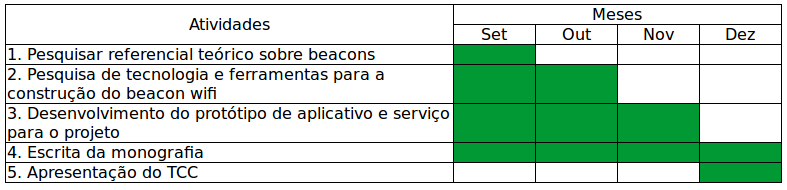
\includegraphics[width=8cm]{figuras/cronograma}}
	}{
	\Fonte{Elaborado pelo autor}			
}	
\end{figure}